%---------------------------------------------------------------------------%
%->> Frontmatter
%---------------------------------------------------------------------------%
%-
%-> 生成封面
%-
\maketitle% 生成中文封面
\MAKETITLE% 生成英文封面
%-
%-> 作者声明
%-
\makedeclaration% 生成声明页
%-
%-> 中文摘要
%-
\intobmk\chapter*{摘\quad 要}% 显示在书签但不显示在目录
\setcounter{page}{1}% 开始页码
\pagenumbering{Roman}% 页码符号

目标跟踪是计算机视觉领域中最重要和最具挑战性的研究课题之一。目标跟踪的核心是估计图像序列的每帧中目标的运动状态。目标跟踪是计算机视觉领域的中层部分,为目标的行为理解提供了基础,因此具有非常重要的理论研究价值。同时,它具有广泛的实际应用,包括视频监控,交通流量监控,视频压缩和人机交互等。例如,目标跟踪已成功应用于监控居民区,停车场和银行中的人类活动(例如W4系统[1]和VSAM项目[2])。在交通运输领域,目标跟踪也被广泛用于交通流量监控[3],行人计数[4]等任务。
由于目标跟踪的理论价值与应用价值,众多科研机构和公司都投入到这项研究中。然而,目标跟踪领域存在很多理论和技术问题有待解决,如运动模糊、光照变化、非刚性目标的形变、视角的变化导致的目标旋转、遮挡等。近年来深度学习的突破为解决目标跟踪中的一系列问题带来了可能。
深度学习是基于人工神经网络的机器学习方法。在过去的十年中,深度学习技术得到了飞速发展,已成功应用于计算机视觉,语音识别,自然语言处理,音频识别,社交网络过滤,机器翻译,生物信息学,药物设计等领域。如何利用深度学习方法,尤其是深度卷积神经网络解决跟踪过程中遇到的复杂问题,具有较大的研究价值和研究空间。

\begin{figure}
\centering
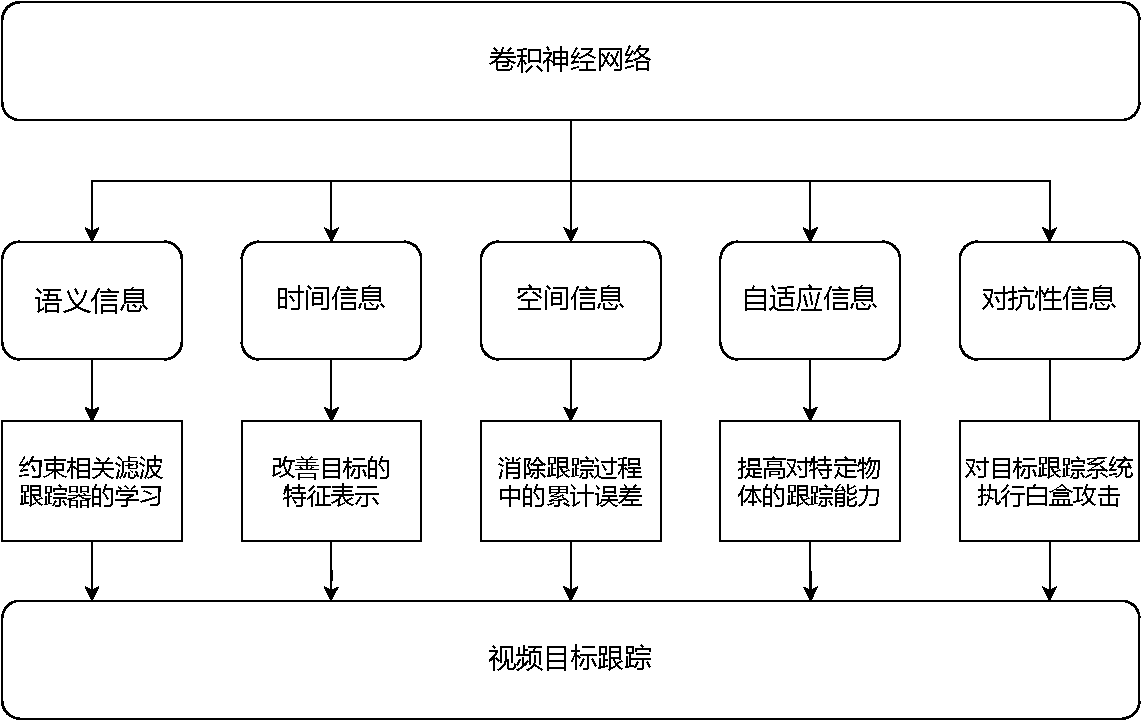
\includegraphics[width=0.75\textwidth]{Img/paper_arch.pdf}
\caption{文章组织架构}
\end{figure}

本文基于卷积神经网络强大的特征提取能力,研究了目标跟踪中的特征鲁棒性。
\begin{itemize}
\item{我们利用卷积神经网络获得目标的\textbf{语义信息}用于约束跟踪器的训练过程,从而提高跟踪的效果。具体而言,我们提出了实例引导的相关滤波器。利用神经网络学习图像的实例级别的语义分割模板约束相关滤波器的学习。}
\item{我们引入了\textbf{时间信息},使得目标表观特征更加丰富,从而提高跟踪的效果。}
\item{现在的算法引入了更丰富的\textbf{空间信息},在空间上是局部搜索的。我们改成了全局搜索。这样的话有利于跟丢之后的找回。}
\item{我们引入了\textbf{自适应信息}提高了算法对特定物体的自适应能力。}
\item{我们引入了\textbf{对抗信息},提出了一种对抗攻击算法,以证明现有跟踪器的鲁棒性不太行。}
\end{itemize}

\keywords{中国科学院大学,学位论文,\LaTeX{}模板}% 中文关键词
%-
%-> 英文摘要
%-
\intobmk\chapter*{Abstract}% 显示在书签但不显示在目录

This paper is a help documentation for the \LaTeX{} class ucasthesis, which is  a thesis template for the University of Chinese Academy of Sciences. The main content is about how to use the ucasthesis, as well as how to write thesis efficiently by using \LaTeX{}.

\KEYWORDS{University of Chinese Academy of Sciences (UCAS), Thesis, \LaTeX{} Template}% 英文关键词
%---------------------------------------------------------------------------%
